\section{Biophysical-Informed System Methodology}
\label{sec:methodology}

The HydroEdge-Net framework bridges physical agro-hydrology and embedded TinyML to enable autonomous, explainable on-device crop water stress diagnosis. This section details the end-to-end mathematical modeling, biophysical feature engineering pipeline, cost-sensitive GBDT formulation, and system architectural workflow.

\subsection{System Architectural Overview}

\begin{figure*}[!t]
\centering
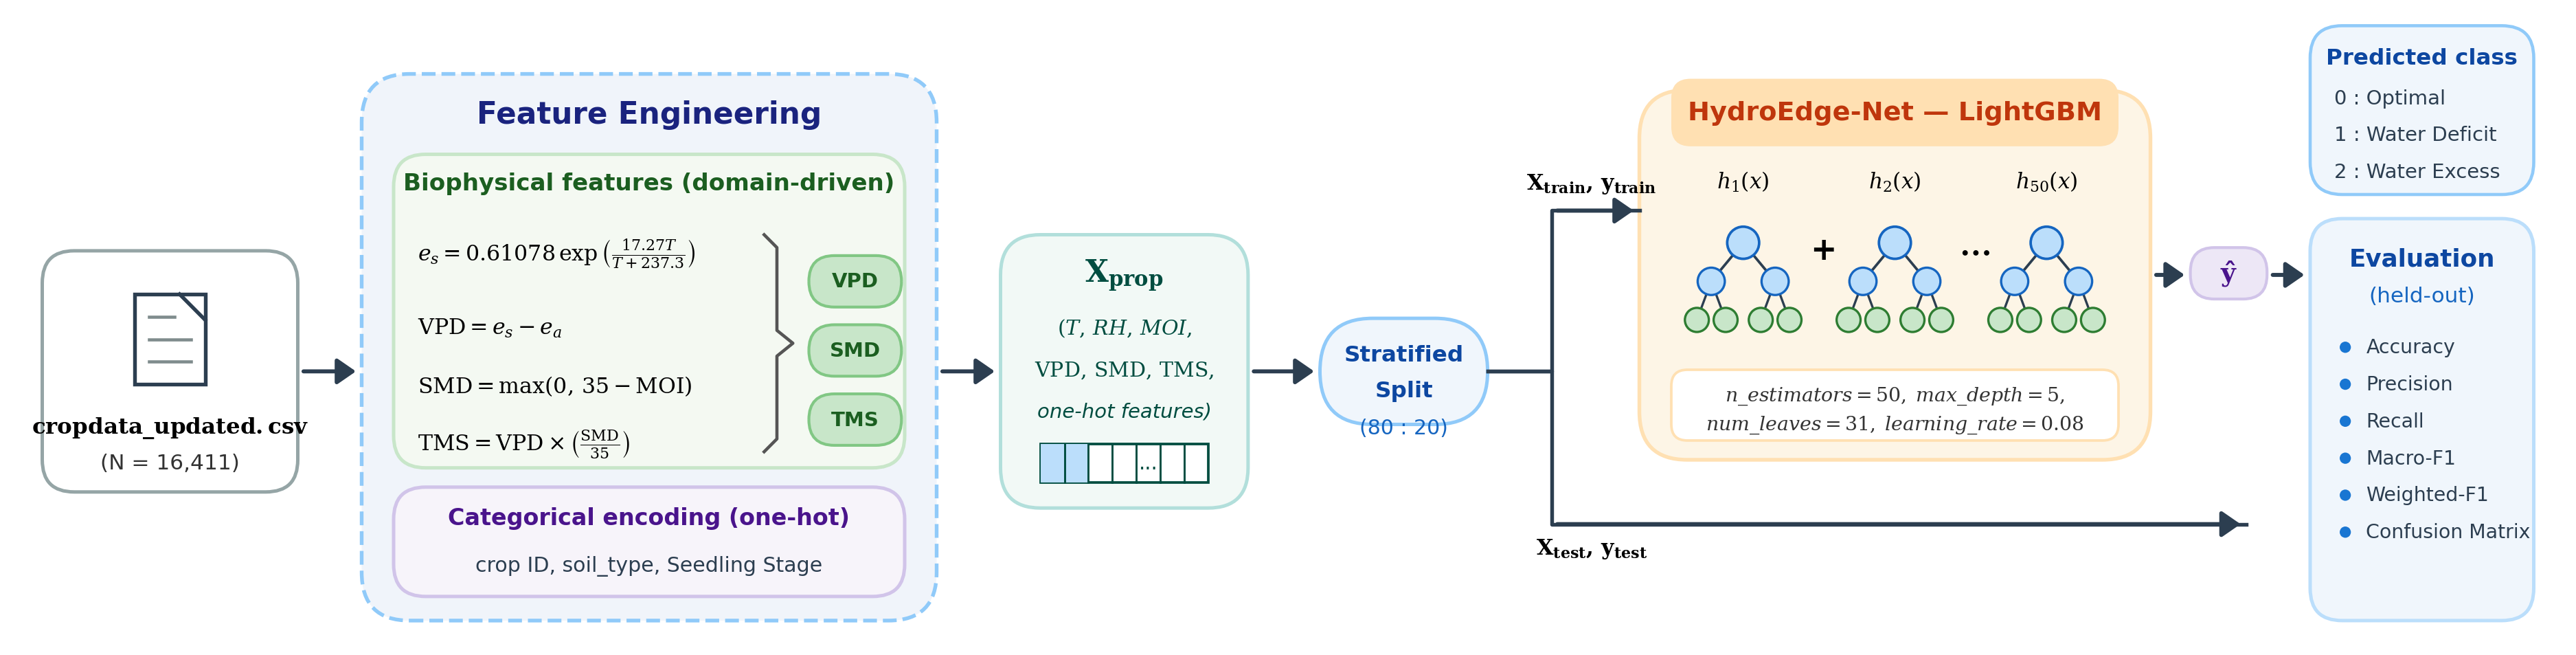
\includegraphics[width=0.98\textwidth]{figures/pipeline_workflow.png}
\caption{End-to-end training and inference pipeline of the HydroEdge-Net framework. Ingesting raw in-situ agricultural telemetry ($N = 16,411$ records), the feature engineering engine calculates domain-driven biophysical features (Tetens VPD, SMD, and non-linear TMS coupling) alongside one-hot categorical encodings, forming the augmented representation $\mathbf{X}_{\text{prop}}$. Data is partitioned via stratified 80:20 splitting into $X_{\text{train}}, y_{\text{train}}$ to train the constrained LightGBM decision tree ensemble ($h_1(x) + \dots + h_{50}(x)$ with depth $\le 5$) and $X_{\text{test}}, y_{\text{test}}$ for held-out multi-metric evaluation across tri-state physiological classes (0: Optimal, 1: Deficit, 2: Excess).}
\label{fig:system_architecture}
\end{figure*}

The holistic architecture of HydroEdge-Net is illustrated in Fig.~\ref{fig:system_architecture}. The framework comprises four interconnected functional tiers:
\begin{enumerate}
    \item \textbf{Multimodal Telemetry Ingestion:} Ingests ambient microclimatic parameters (air temperature $T$, relative humidity $\text{RH}$) and edaphic variables (volumetric soil moisture content $\theta$) at periodic intervals (e.g., once every 15 minutes).
    \item \textbf{Biophysically Informed Edge Engine:} Rather than passing raw numerical sensor streams to the classifier, an ultra-lightweight arithmetic module computes the atmospheric vapor pressure deficit, edaphic moisture depletion, and coupled thermal-moisture stress index, augmented by categorical encodings for soil hydraulic conductivity and phenological sensitivity.
    \item \textbf{Constrained Cost-Sensitive TinyML Classifier:} The engineered feature vector is evaluated by an ensemble of shallow decision trees ($d \le 5$, 45 estimators) optimized via class-weighted gradient boosting. The decision tree topology is statically compiled into pure C routines without heap allocation.
    \item \textbf{Closed-Loop Scheduling and Explainable Validation:} The output classifies crop water status into three mutually exclusive agronomic regimes: \textit{Class 0 (Optimal Moisture)}, \textit{Class 1 (Water Deficit Stress)}, and \textit{Class 2 (Excess Saturated Water)}. Upon diagnosing Class 1, autonomous irrigation dosing is triggered to replenish the crop root zone. Furthermore, feature attribution analysis via TreeSHAP provides transparent interpretability, confirming that predictions are anchored in valid agro-hydrological dynamics.
\end{enumerate}

\subsection{Biophysical Feature Engineering Formulations}

A central premise of HydroEdge-Net is that direct integration of biophysical domain knowledge dramatically reduces the hypothesis space required by machine learning algorithms, enabling ultra-compact decision trees to outperform unconstrained heavy neural networks.

\subsubsection{Atmospheric Evaporative Demand (VPD)}
Plants respond not to ambient temperature or relative humidity in isolation, but to the atmospheric vapor pressure deficit (VPD)---the physical drying power of the atmosphere that governs transpirational flux across stomata~\cite{monteith1965evaporation}. Using Tetens' formulation~\cite{tetens1930uber}, the saturation vapor pressure $e_s(T)$ at ambient air temperature $T$ ($^{\circ}\text{C}$) is formulated as:
\begin{equation}
e_s(T) = 0.61078 \exp\left( \frac{17.27 \times T}{T + 237.3} \right) \quad [\text{kPa}]
\label{eq:tetens_es}
\end{equation}
The actual ambient vapor pressure $e_a(T, \text{RH})$ is a function of saturation pressure and relative humidity $\text{RH}$ (\%):
\begin{equation}
e_a(T, \text{RH}) = e_s(T) \times \left( \frac{\text{RH}}{100} \right) \quad [\text{kPa}]
\label{eq:tetens_ea}
\end{equation}
The instantaneous atmospheric Vapor Pressure Deficit ($\text{VPD}$) is the difference between saturation and actual vapor pressures:
\begin{align}
\text{VPD} &= e_s(T) - e_a(T, \text{RH}) \nonumber \\
&= e_s(T) \times \left( 1 - \frac{\text{RH}}{100} \right) \quad [\text{kPa}]
\label{eq:vpd}
\end{align}
High VPD ($>1.5$~kPa) induces substantial atmospheric pull on leaf moisture, forcing stomatal closure to prevent cavitation even under moderate soil moisture.

\subsubsection{Edaphic Soil Moisture Deficit (SMD)}
Volumetric soil moisture content $\theta$ (\%) must be evaluated against the soil-specific field capacity ($\theta_{\text{FC}}$), defined as the upper limit of water retained against gravitational drainage after free drainage has ceased~\cite{allen1998crop}. For standard agricultural soils (loam and silt-clay loam profiles), the baseline field capacity is anchored at $\theta_{\text{FC}} = 35.0\%$. The instantaneous Soil Moisture Deficit ($\text{SMD}$) is quantified as:
\begin{equation}
\text{SMD} = \max\left(0, \, \theta_{\text{FC}} - \theta\right) \quad [\%]
\label{eq:smd}
\end{equation}
When $\theta \ge \theta_{\text{FC}}$, $\text{SMD} = 0$, indicating that soil moisture is at or above field capacity. When $\theta < \theta_{\text{FC}}$, $\text{SMD}$ provides a normalized measure of the volumetric soil water deficit required to replenish the root zone.

\subsubsection{Thermal-Moisture Stress Coupling Index \texorpdfstring{($\Psi_{\text{TMS}}$)}{(Psi\_TMS)}}
In classical crop ecophysiology, plants maintain transpirational evaporative cooling under elevated atmospheric VPD only if sufficient soil water is available in the root zone~\cite{jackson1981canopy, idso1981normalizing}. When atmospheric demand is elevated (high VPD) while root-zone moisture is severely depleted (high SMD), stomatal conductance drops abruptly to protect the xylem conduit, causing rapid canopy overheating and cellular desiccation. To capture this multiplicative, highly nonlinear physiological strain without requiring expensive infrared thermal cameras, we formulate the \textbf{Thermal-Moisture Stress Coupling Index} ($\Psi_{\text{TMS}}$) as:
\begin{equation}
\Psi_{\text{TMS}} = \text{VPD} \times \left( \frac{\text{SMD}}{\theta_{\text{FC}}} \right) \quad [\text{kPa}]
\label{eq:tms}
\end{equation}
where $\text{SMD} / \theta_{\text{FC}}$ represents the fractional soil water depletion. Under non-stress conditions ($\text{SMD} \to 0$), $\Psi_{\text{TMS}} \to 0$ even during hot midday periods, accurately capturing that well-watered crops continue active transpirational cooling. Conversely, when severe atmospheric dryness coincides with depleted soil moisture reserves, $\Psi_{\text{TMS}}$ scales multiplicatively, providing an early diagnostic trigger for water deficit stress.

\subsubsection{Categorical Soil and Phenological Encodings}
Hydraulic conductivity and crop vulnerability to water stress vary significantly across soil textures and developmental stages~\cite{wu2026agpstc}. HydroEdge-Net incorporates integer-encoded categorical vectors:
\begin{itemize}
    \item \textbf{Soil Texture Encodings ($S \in \{0, \dots, 6\}$):} Representing seven distinct textural classes (Black, Alluvial, Sandy, Red, Clay, Loam, Chalky), each governing intrinsic matric potential, hydraulic conductivity, and wilting points.
    \item \textbf{Phenological Stage Encodings ($P \in \{0, \dots, 7\}$):} Representing eight developmental phases (Germination, Seedling, Vegetative, Flowering, Pollination, Fruit Formation, Maturation, Harvest). Critical phases such as Flowering and Fruit Formation carry heightened yield sensitivity to drought stress.
\end{itemize}

The resulting engineered feature vector supplied to the classifier is:
\begin{equation}
\mathbf{x} = \left[ T, \, \text{RH}, \, \theta, \, \text{VPD}, \, \text{SMD}, \, \Psi_{\text{TMS}}, \, S, \, P \right]^T \in \mathbb{R}^8
\label{eq:feature_vector}
\end{equation}

\subsection{Constrained Cost-Sensitive TinyML Formulation}

For edge microcontroller deployment, the classification model must satisfy strict bounds: (i) deterministic sub-5~ms execution latency, (ii) Flash footprint $<30$~KB, and (iii) SRAM usage $<16$~KB. To fulfill these constraints, HydroEdge-Net employs a constrained Gradient Boosted Decision Tree (GBDT) based on the LightGBM architecture~\cite{ke2017lightgbm}.

\subsubsection{Leaf-Wise Tree Growth with Strict Depth Constraints}
Unlike standard depth-wise tree algorithms that split all nodes level-by-level, LightGBM uses leaf-wise (best-first) tree growth, selecting the leaf that yields the maximum loss reduction. To prevent overfitting and restrict stack depth on 32-bit MCUs, we impose strict structural bounds:
\begin{equation}
d \le 5, \quad N_{\text{leaves}} \le 31, \quad N_{\text{trees}} = 45
\label{eq:tree_bounds}
\end{equation}
Bounding tree depth to $d \le 5$ guarantees that the worst-case branch execution path per tree requires at most 5 comparative operations, bounding total inference cycles to $45 \times 5 = 225$ comparison instructions.

\subsubsection{Cost-Sensitive Loss Reweighting}
In agricultural datasets, non-stress instances (optimal moisture) constitute the overwhelming majority of operating hours, while water deficit stress and extreme saturation are minority occurrences. Unweighted cross-entropy loss leads to model bias toward the majority class, causing unacceptably high false-negative rates on water deficit stress (crop desiccation). To rectify this imbalance, we introduce class-specific loss weights $\omega_k$ during ensemble training:
\begin{equation}
\omega_k = \frac{N_{\text{majority}}}{N_k} = \frac{\max_{j} N_j}{N_k}
\label{eq:cost_weight}
\end{equation}
where $N_k$ denotes the sample count for class $k \in \{0, 1, 2\}$. For a training sample $(\mathbf{x}_i, y_i)$, the multi-class negative log-likelihood objective function is weighted as:
\begin{equation}
\mathcal{L} = -\sum_{i=1}^{N} \sum_{k=0}^{2} \omega_k \cdot \mathbb{I}(y_i = k) \ln p_k(\mathbf{x}_i) + \sum_{m=1}^{M} \Omega(f_m)
\label{eq:weighted_loss}
\end{equation}
where $p_k(\mathbf{x}_i)$ is the predicted probability for class $k$, $\mathbb{I}(\cdot)$ is the indicator function, and $\Omega(f_m) = \gamma N_{\text{leaves}} + \frac{1}{2} \lambda \sum w_j^2$ is the tree complexity regularization term with penalization parameters $\gamma$ and $\lambda$. By heavily penalizing errors on the minority deficit class ($\omega_1 \gg 1$), the model prioritizes sensitivity to drought stress, ensuring that soil water depletion is intercepted prior to wilting.
